\section{Reconocimiento de elementos en laboratorio}
\label{sec:laboratorio}
La \autoref{tab:laboratorio} relaciona los elementos disponibles en el laboratorio con su función, su ubicación dentro de la red diseñada y los componentes seleccionados en la \autoref{sec:componentes}.

\begin{longtable}{|p{2.4cm}|p{3.5cm}|p{3.2cm}|p{4.6cm}|}
    \caption{Elementos del laboratorio, su función y su ubicación en la red.}\label{tab:laboratorio}\\
    \hline
    \textbf{Elemento} & \textbf{Función} & \textbf{Ubicación en la red} & \textbf{Instalación y manipulación} \\
    \hline
    \endfirsthead
    \hline
    \textbf{Elemento} & \textbf{Función} & \textbf{Ubicación en la red} & \textbf{Instalación y manipulación} \\
    \hline
    \endhead
    Cable troncal de tubos holgados & Transportar las fibras desde el hub hasta los clusters & Postes, desde el hub hasta las CEO de cluster & Respetar el radio de curvatura ($20 \times D$ durante el tendido) y la tracción máxima; dejar rulos de reserva en las cajas \\
    \hline
    Cable de distribución (tubo central) & Llevar las fibras de la caja de distribución a las CTO & Postes dentro de cada sector & Abrir el tubo solo en la ventana de la caja (sangría) sin dañar las fibras que siguen de paso \\
    \hline
    Cable drop & Conectar la CTO con la vivienda & Entre el poste de la CTO y la fachada & Retirar el mensajero de acero solo en los extremos; fibra G.657.A, tolera curvaturas cerradas \\
    \hline
    Conectores y adaptadores SC/APC & Unión desmontable entre fibras & ODF, CTO, roseta y ONT & Inspeccionar y limpiar la férula antes de cada conexión; no mezclar APC (verde) con UPC (azul) \\
    \hline
    Pigtails y patch cords & Terminar fibras en paneles y conectar equipos & ODF del hub y domicilio & Empalmar los pigtails por fusión; no exceder el radio de curvatura en los organizadores \\
    \hline
    Splitter PLC & Dividir la potencia óptica entre varias salidas & Caja de distribución (1:4) y CTO (1:16) & Su pérdida aumenta con la relación de división (aprox. $10 \log N$ más la pérdida en exceso) \\
    \hline
    Caja de empalme (CEO) & Proteger empalmes y derivaciones & Derivaciones del troncal y cajas de distribución & Cierre hermético; ordenar las fibras en bandejas y respetar el radio mínimo de $30 \, [mm]$ \\
    \hline
    Caja terminal (CTO/NAP) & Punto de conexión de los drops & Postes, una por cada grupo de hasta 17 viviendas & Identificar cada salida; sellar los pasacables no utilizados \\
    \hline
    Empalmadora por fusión & Unir fibras con baja pérdida & Todas las cajas de empalme & Pelado, limpieza con alcohol isopropílico y corte con cortadora de precisión; descartar los restos de fibra en un recipiente \\
    \hline
    Localizador visual de fallas (VFL) & Verificar continuidad e identificar fibras & Mantenimiento y puesta en servicio & No mirar directamente el haz \\
    \hline
    Medidor de potencia óptica & Medir la potencia recibida & Puesta en servicio: salida de la CTO y roseta & Seleccionar la longitud de onda de calibración que corresponde a la señal medida \\
    \hline
    Peladora y cortadora de precisión & Retirar los recubrimientos y obtener un corte plano de la fibra & Preparación de todo empalme o conector & Respetar las longitudes de pelado y corte del accesorio; limpiar con alcohol isopropílico antes de cortar \\
    \hline
    Conector y empalme mecánicos & Terminar o unir fibras en campo sin empalmadora & Reparaciones de emergencia y acometidas & Empalme 3M Fibrlok II con herramienta 2501; insertar la fibra hasta formar el arco de control y proteger el empalme \\
    \hline
\end{longtable}

\subsection{Prácticas realizadas}
\label{sec:practicas_lab}
Las prácticas indicadas por la cátedra se realizaron con las herramientas de instalación del laboratorio, y su desarrollo completo se presenta en la Parte 2 del Trabajo Práctico N.° 3 \cite{informe_tp3}. A continuación se resumen los resultados y su relación con la red diseñada.

\textbf{Práctico A, detección visual de fallas:} se acopló el VFL a un tramo de cable y la luz roja apareció como un punto definido en el extremo opuesto, lo que confirmó la continuidad del hilo (\autoref{fig:lab_vfl}). Al medir esa luz con el medidor de potencia se obtuvo un valor distinto de cero pero no confiable, porque el VFL emite en $650 \, [nm]$ y la menor longitud de onda seleccionable en el medidor era $800 \, [nm]$: la respuesta del fotodetector depende de $\lambda$, y fuera de la longitud de onda de calibración la lectura solo indica presencia de señal.

\begin{figure}[H]
    \centering
    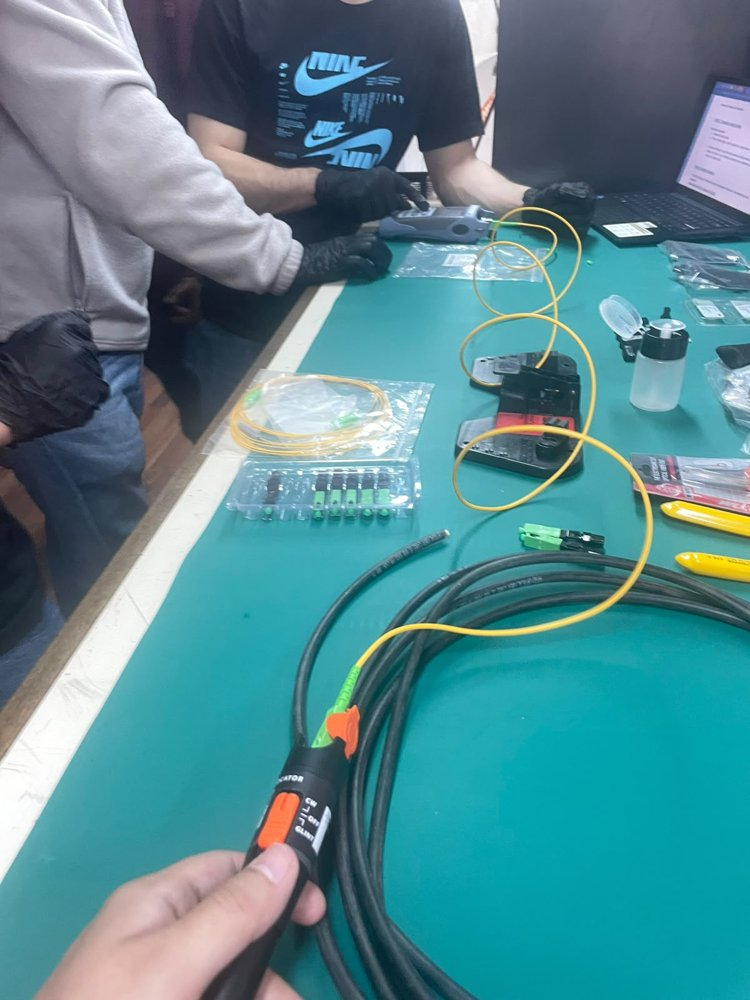
\includegraphics[width=0.28\textwidth]{lab_vfl_continuidad.jpg}
    \caption{Verificación de continuidad con el VFL y el medidor de potencia. Fuente: Trabajo Práctico N.° 3 \cite{informe_tp3}.}
    \label{fig:lab_vfl}
\end{figure}

\textbf{Práctico B, conectorización mecánica SC/APC:} se peló el cable, se limpió la fibra, se cortó a $10 \, [mm]$ con la cortadora de precisión y se insertó en el conector hasta formar el arco de control, que indica contacto contra el tope interno (\autoref{fig:lab_conector}). Se necesitaron varios intentos porque la fibra se quebraba durante la preparación. El conector quedó armado, pero el medidor de potencia no registró señal.

\begin{figure}[H]
    \centering
    \begin{subfigure}{0.22\textwidth}
        \centering
        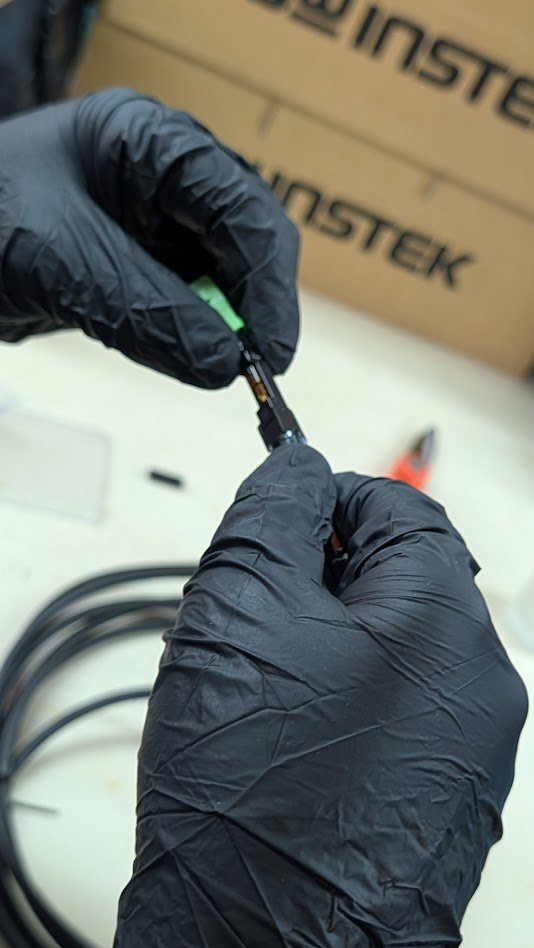
\includegraphics[width=\linewidth]{lab_conector_insercion.jpg}
        \caption{Inserción de la fibra cortada.}
    \end{subfigure}
    \hspace{1cm}
    \begin{subfigure}{0.30\textwidth}
        \centering
        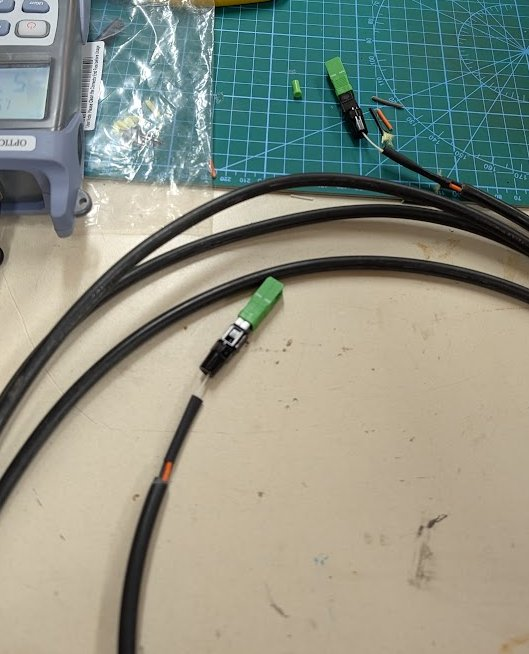
\includegraphics[width=\linewidth]{lab_conector_sc_apc.jpg}
        \caption{Conector SC/APC armado.}
    \end{subfigure}
    \caption{Montaje del conector mecánico SC/APC. Fuente: Trabajo Práctico N.° 3 \cite{informe_tp3}.}
    \label{fig:lab_conector}
\end{figure}

\textbf{Práctico C, empalme mecánico:} con la herramienta 3M 2501 se prepararon dos fibras (pelado, limpieza y corte a $12{,}5 \, [mm]$), se insertaron en el módulo de empalme hasta igualar los arcos y se cerró la tapa, que fija la alineación con gel adaptador de índice. Luego se colocó un protector sobre el empalme (\autoref{fig:lab_empalme}). Como se usó el mismo cable del práctico anterior, el medidor tampoco registró potencia. La falla se atribuyó a una rotura de la fibra en un punto del cable que no pudo ubicarse con el VFL, porque las capas de cubierta impedían ver la fuga de luz.

\begin{figure}[H]
    \centering
    \begin{subfigure}{0.30\textwidth}
        \centering
        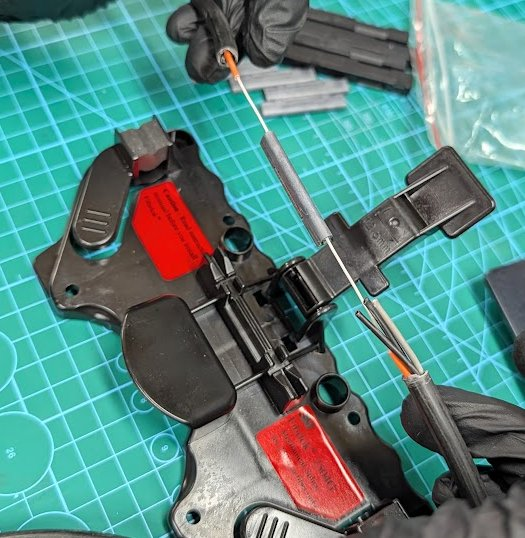
\includegraphics[width=\linewidth]{lab_empalme_mecanico.jpg}
        \caption{Empalme terminado.}
    \end{subfigure}
    \hfill
    \begin{subfigure}{0.62\textwidth}
        \centering
        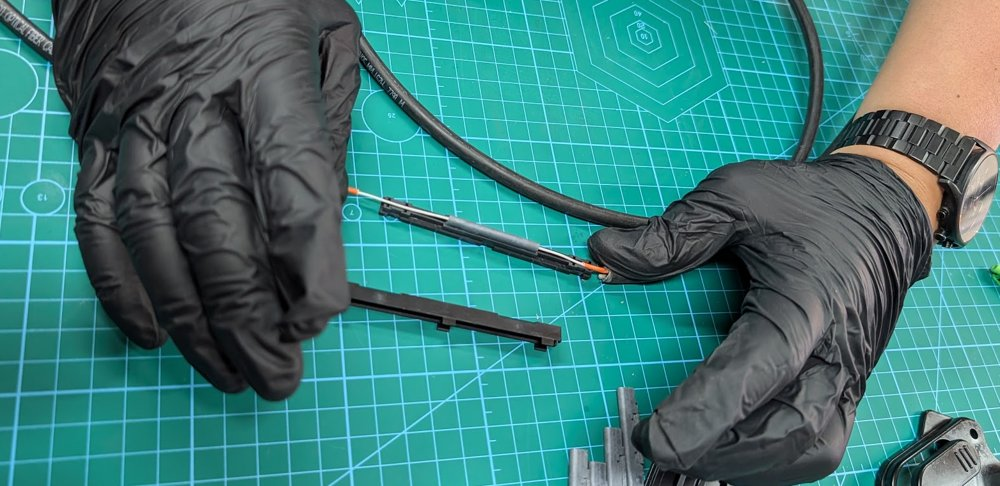
\includegraphics[width=\linewidth]{lab_empalme_protector.jpg}
        \caption{Colocación del protector.}
    \end{subfigure}
    \caption{Ejecución del empalme mecánico. Fuente: Trabajo Práctico N.° 3 \cite{informe_tp3}.}
    \label{fig:lab_empalme}
\end{figure}

\subsection{Vínculo con la Actividad N.° 3 y con el diseño}
En la Parte 1 de la Actividad N.° 3 se comprobó que la potencia que llega al receptor disminuye con la longitud de la fibra y con los acoplamientos imperfectos (al enfrentar los conectores a mano la señal se escuchaba más débil), y que el receptor digital deja de recuperar la señal cuando esta no supera su umbral \cite{informe_tp3}. En una red GPON el mismo principio se cuantifica con el presupuesto óptico: los splitters, conectores y empalmes reconocidos en el laboratorio son los eventos de pérdida que se suman en la \autoref{sec:presupuesto}, y la sensibilidad de la ONT y de la OLT cumple el papel del umbral de decisión.

Las prácticas de instalación respaldan las siguientes decisiones del diseño:
\begin{itemize}
    \item \underline{Empalmes por fusión en la planta externa:} la fragilidad observada al preparar la fibra a mano, y la falla que dejó el enlace sin señal, muestran que la calidad depende del operador. Un empalme mecánico bien ejecutado tiene una pérdida típica menor a $0{,}1 \, [dB]$, pero su reflectancia puede llegar a $-35 \, [dB]$ en todo el rango de temperatura \cite{fibrlok}, mientras que la fusión no tiene interfaz de gel y es permanente. Por eso el diseño adopta empalmes por fusión en las CEO, las cajas de distribución, la entrada de las CTO y la roseta, y reserva los empalmes mecánicos para reparaciones de emergencia. En el extremo del drop que se conecta a la salida SC/APC de la CTO se recomienda usar drops preconectorizados de fábrica; si se usan conectores mecánicos de campo como el del práctico B, cada acometida debe verificarse con el medidor de potencia al instalarla.
    \item \underline{Margen de ingeniería y reservas de cable:} cada reparación agrega empalmes, y en el laboratorio fueron necesarios varios intentos para obtener un corte correcto. El margen de $3 \, [dB]$ y los rulos de reserva de $20 \, [m]$ por caja de empalme y $10 \, [m]$ por CTO (\autoref{sec:trazas}) permiten rehacer empalmes sin reemplazar el cable.
    \item \underline{Instrumental de puesta en servicio:} el medidor de potencia debe estar calibrado en las longitudes de onda de la red ($1310$, $1490$ y, con video overlay, $1550 \, [nm]$), ya que fuera de ellas la lectura no es válida. El VFL sirve para verificar continuidad e identificar fibras en las cajas, pero no localiza roturas dentro de cables con cubierta: para eso se requiere un reflectómetro (OTDR), con el que deben certificarse los tramos al construir la red.
\end{itemize}
